\section{\uppercase{Results}}
\label{sec:results}
\noindent All 96 method/case slots were attempted. Table~\ref{tab:outcomes} and Figure~\ref{fig:results} are generated directly from frozen machine-readable reports. Enumeration answered \EnumVisible/24 questions completely through its own selections. A produced \AVisible/24 complete visible answers, B \BVisible/24, and C \CVisible/24. Model-selected completeness was \ASelected/24, \BSelected/24, and \CSelected/24, respectively. These frozen values include the scoring caveat discussed below; they are not newly adjudicated accuracy estimates.\draftassist

\begin{table*}[!t]
\caption{Frozen outcomes. Every main endpoint retains all 24 cases per condition. ``Selected complete'' excludes compiler-supplied requested answers; enumeration's selections are deterministic. ``Both insuff.'' uses the four cases requesting separate personal and peer insufficiency answers. B's completeness has the answer-form caveat in Section~\ref{sec:caveat}.}
\label{tab:outcomes}
\centering\setlength{\tabcolsep}{4pt}
%% Generated from frozen reports; do not edit.
\begin{tabular}{lrrrrr}
\hline
Condition & First valid & Accepted & Visible complete & Selected complete & Both insuff. answers \\
\hline
Enumeration & 24/24 & 24/24 & 24/24 & 24/24 & 4/4 \\
A: compact & 21/24 & 22/24 & 21/24 & 18/24 & 3/4 \\
B: derived metadata & 22/24 & 24/24 & 15/24 & 14/24 & 2/4 \\
C: explicit binding & 21/24 & 21/24 & 15/24 & 11/24 & 1/4 \\
\hline
\end{tabular}

\end{table*}

\begin{figure*}[!t]
\centering
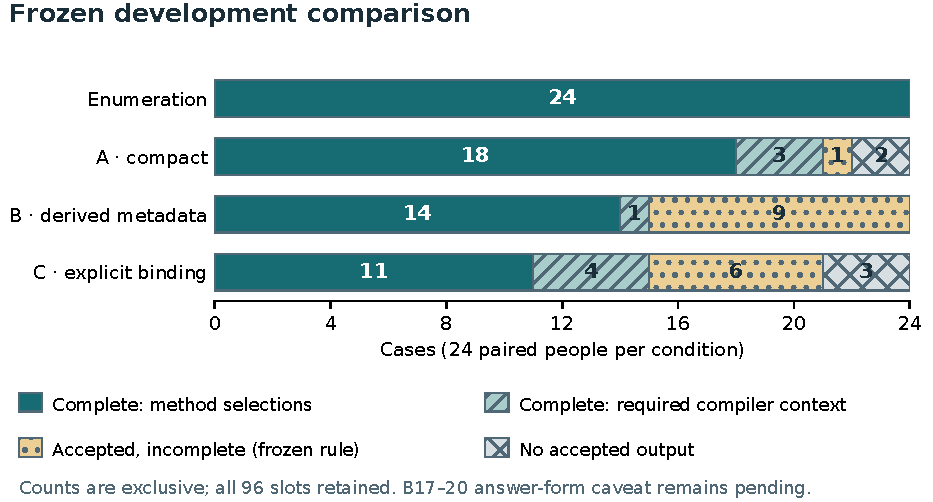
\includegraphics[width=\textwidth]{figures/results.pdf}
\caption{Frozen development comparison on 24 paired people. Categories are mutually exclusive: complete through method selections; otherwise complete with required compiler context; otherwise accepted but incomplete; or no accepted output. All numbers, even in model-selected answers, come from deterministic tools. B17--20 visibly contain requested recent means in personal-change claims that the frozen focal predicate does not credit. These four cases remain in the incomplete category pending human adjudication. No score is revised here.}
\label{fig:results}
\end{figure*}

\subsection{Validity, Completeness and Attribution}
B achieved 24 accepted outputs, compared with 22 for A and 21 for C, but its frozen visible completeness remained lower than A's. Successful final repairs were one of three for A, two of two for B, and zero of three for C. Rejections remained in the denominator; there were no infrastructure-blocked episodes or deterministic fallbacks. No agent met the combined engineering target.

Compiler-supplied requested context completed three additional A cases, one B case, and four C cases. Its 32, 37, and 37 added panels contained no added comparison or personal-change claim. Panel count is not a quality score. Supplied grade limitations, for example, can answer a request without model selection.

In paired outcomes (Table~\ref{tab:paired}), C loses six visible complete cases relative to A and has no net gain over B: three improve and three regress. Selected completeness is seven below A and three below B. These frozen results do not support a binding benefit; disputed B judgments qualify the equality with C.

\begin{table}[t]
\caption{Paired visible completeness on the same 24 people. ``Right only'' and ``Left only'' refer to the named contrast. Counts are descriptive, with no significance test.}
\label{tab:paired}
\centering\setlength{\tabcolsep}{3pt}
%% Generated from frozen reports; do not edit.
\begin{tabular}{lrrrr}
\hline
Right $-$ left & Both & Right only & Left only & Neither \\
\hline
C $-$ A & 14 & 1 & 7 & 2 \\
C $-$ B & 12 & 3 & 3 & 6 \\
B $-$ A & 14 & 1 & 7 & 2 \\
\hline
\end{tabular}

\end{table}

\subsection{Evidence Retrieval and Failure Mechanisms}
The offline diagnostic found sufficient returned evidence for all 24 questions in both A and B, and 21 in C. In case~15, A nevertheless selected peer comparisons for weeks~0--3 when asked about weeks~10--11. Returned recent evidence supported a separate personal-insufficiency answer, but its peer answer was omitted (Figure~\ref{fig:failure}). Correct earlier-window binding does not establish relevance.

C12 selected an earlier result for a requested recent mean. Invalid C18--20 analysis batches returned no evidence; final/repair handles remained unresolved. No catalogue had been returned, so its contents alone cannot explain those failures. A09 repaired peer selections paired with personal conclusion scope; A12 did not. A22 retained invalid scope; B23 repaired a panel-limit error. These are trace observations, not established cognitive causes.

All 168 comparison generations reached end-of-sequence, with at most 491 output tokens: failures were not output-limit truncation. Source checks detected no accepted unsupported quantitative answer among 91 accepted dashboards. This bounded result establishes agreement with checked fields/support rules, not universal semantic correctness or completeness.

\subsection{Unresolved Answer-Equivalence Caveat}
\label{sec:caveat}
B17--20 display both requested recent assessment means within supported personal-change claims. The frozen focal-item predicate recognizes a comparison panel or a supported comparison claim, but does not inspect a personal-change claim for that mean. It therefore classifies eight requested items as retrieved but omitted even though their feature, units, recent window, and values appear on the page. This is an evaluation representation limitation, not a numerical failure. B remains 15/24 visible complete and 14/24 selected complete in every reported table and figure; no disputed case receives new credit.

C21/C23 display earlier and recent means in peer claims without an explicit personal-change answer; equivalence is a separate unresolved question. Unavailable forms and scoped insufficiency also require review. All 96 original slots, including rejections, are prepared for two reviewers and adjudication, but no ratings exist. Automated inspection is not independent human review, and frozen completeness is not a settled measurement construct.

\begin{figure*}[!t]
\centering
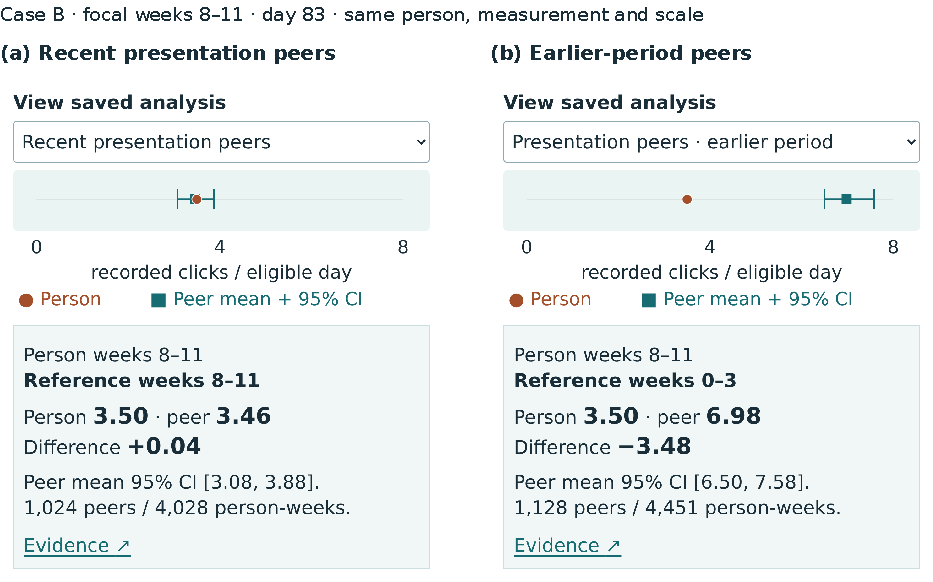
\includegraphics[width=\textwidth]{figures/reference_switch.pdf}
\caption{A saved reference-period change in condition A, case~05. Both comparisons were model-selected. Browser excerpts show the selector reading validated records, not recomputing statistics. The person, focal weeks~8--11, units, and scale stay fixed; the reference changes from weeks~8--11 to weeks~0--3. Eligible membership differs (1,024 versus 1,128 people). Whiskers are 95\% bootstrap intervals for peer means, not for contrasts. The later presentation layer supplies the layout. Earlier peers are not necessarily fairer or causally adjusted.}
\label{fig:reference}
\end{figure*}

\subsection{Recorded Cost}
Table~\ref{tab:costs} retains failures and repairs. Enumeration used more calls but far less episode time and no inference. C used more generations and equivalent repeated analyses than either control without higher completeness. This supports enumeration's operational economy within the registry.

\begin{table*}[!t]
\caption{Recorded comparison costs summed over 24 cases per condition. Episode time includes analytical and rendering work; shared model loading/profiling is separate. $^{a}$Exact/equivalent repeated requests use the frozen signatures; equivalent requests share feature, group and window meaning. Input/output token totals count repeated context, failures, and repairs.}
\label{tab:costs}
\centering\setlength{\tabcolsep}{3pt}
%% Generated from frozen reports; do not edit.
\begin{tabular}{lrrrrrr}
\hline
Condition & Tools & Repeated$^{a}$ & Generations & Input / output tokens & Episode s & Median s \\
\hline
Enumeration & 84 & 0 / 0 & 0 & 0 / 0 & 35.40 & 1.18 \\
A: compact & 76 & 0 / 5 & 52 & 178,794 / 10,274 & 484.64 & 17.07 \\
B: derived metadata & 79 & 0 / 8 & 53 & 238,675 / 10,012 & 504.21 & 16.87 \\
C: explicit binding & 82 & 4 / 12 & 63 & 262,031 / 10,695 & 536.32 & 21.19 \\
\hline
\end{tabular}

\end{table*}

Including setup/construction, 185 generations used 1,719.02~s of model-process time (28.65~min), including loading/cleanup: 153.02~s construction and 1,566.00~s comparison. Shared comparison loading/profiling took 37.55/1.65~s. Peak allocated/reserved memory was 30.78/35.23~GiB; maximum input was 10,888 tokens. Process time, episode latency, and implementation wall time differ and do not establish billing time. Manuscript preparation ran no experimental inference.
